\documentclass[a4paper, 10pt]{article} 
\usepackage[brazil]{babel} 
\usepackage[utf8]{inputenc} 
\usepackage{amssymb, amsmath, pxfonts}
\usepackage{mathrsfs} 
\usepackage[normalem]{ulem}  
\usepackage{mathrsfs}  \usepackage[top=2cm,left=3cm,right=2cm,bottom=3cm]{geometry}  \usepackage{graphicx} 
\usepackage[usenames]{color} 
\usepackage[utf8]{inputenc}
\usepackage{graphicx}
\usepackage{wrapfig}
\usepackage{float}
\usepackage{multirow}
\usepackage{tabularx}

\title{ Algoritmo em Grafos}
\author{Mateus Dutra Santiago}
\date{April 2019}

\begin{document}

\maketitle

\section{Introdução}
\quad Quando se falam em grafos, refere-se a um conjunto de pontos, que são denominados vértices, que são ligados por linhas, denominadas arestas. Traduzindo para uma linguagem mais formal \textit{"Um grafo é um conjunto não vazio de nós (vértices) e um conjunto de arcos (arestas) em que
cada arco conecta dois nós."~\cite{J}}
\begin{figure}[!htb]
    \center
    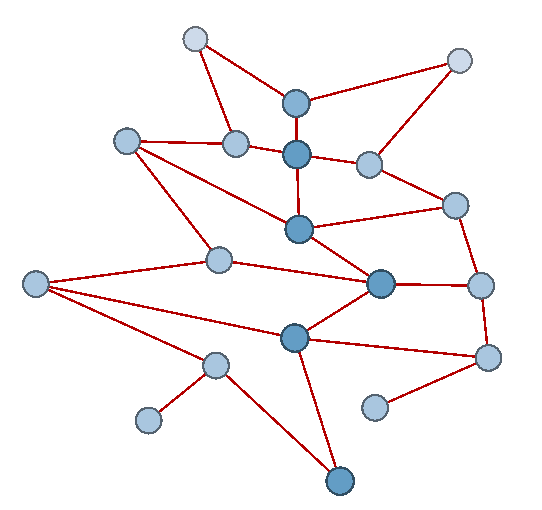
\includegraphics[width=5cm, height=6cm, angle=0]{mateus_dutra1.png}
    \caption{\label{fig:my-label} Esse é um exemplo de um grafo.}
\end{figure}

\quad Apesar da Teoria dos Grafos ser basear principalmente na base teorica da matemática \textit{que estuda as relações entre os objetos de um determinado conjunto}~\cite{tg}, os grafos também podem ser usados para a construção de algoritmos, que são um conjunto de instruções que segue uma lógica embasada para a solução de um determinado problema, visto que textit{a maioria dos problemas é naturalmente formulada em termos de objetos e as conexões entre eles.}~\cite{RS}

\quad Circuitos eletricos também são um exemplo em que as interconexões entre objetos desempenham um papel central.
\section{Relevância}
\quad \textit{Embora a ideia de um gráfico seja muito simples, um número surpreendente de situações tem relações entre itens que se prestam à representação gráfica.}~\cite{J}Sendo assim, os grafos não são usados apenas na área da matemática teorica, abrangendo muitas outras áreas, participando de forma consistente no cotidiano da população, como por exemplo, em circuitos elétricos, nas rotas de aviões, e até mesmo na representação gráfica de moléculas.
\begin{figure}[H]
    \centering
    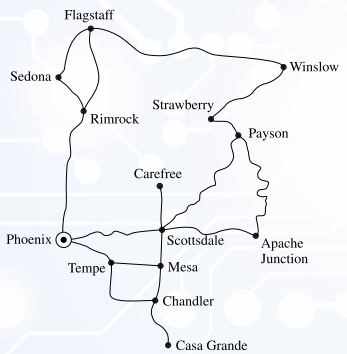
\includegraphics[width=6cm, height=8cm, angle=0]{mateus_dutra2.png}
    \caption{\label{fig:arizona} Esse é um mapa das estradas do Arizona, um exemplo básico do uso de grafos no cotidiano.}
\end{figure}
\quad Portanto, os grafos também possuem atuação direta na computação, apesar de não tão visível quanto as demais, sendo usado principalmente na forma de algoritmo com o intuito de encontrar o caminho “mais curto” de um nó para outro no grafo, em outras palavras, realizar os passos que formentem uma escolha mais eficiente.
\section{Relação com outras disciplinas}
 \begin{table}[H]
\centering
\begin{tabular}{|l|l|}
\hline
Matéria & Relação \\ \hline
\begin{tabular}[c]{@{}l@{}}CC0105 - Fundamentos de Matemática \\ Discreta\end{tabular} & \begin{tabular}[c]{@{}l@{}}Primordialmente, vemos a relação na nomenclatura, \\ já que a Matemática Discreta é também nomeada \\ como Matemática Finita, e assim,é possível construir\\ um paralelo com os grafos, já que todo grafo, independente\\ de quão grande seja, é finito. Logo é possível afirmar que a\\  Teoria do Grafos é uma subdivisão da Matemática Discreta.\end{tabular} \\ \hline
{\begin{tabular}[c]{@{}l@{}}CC0201 Algoritmos e Estruturas \\ de Dados I\end{tabular}} & {\begin{tabular}[c]{@{}l@{}}Como já dito anteriormente, a maioria dos problemas é \\ naturalmente formulada em termos de objetos e as conexões\\ entre eles, portanto a estratégia e argumentação utilizadas \\ para "solucionar" esses problemas também deve utilizar dos \\ objetos e das conexões entre eles, o que éo cerne da Teoria \\ dos Grafos. Além disso, na computação,os dados são tidos\\ como um conjunto de valores ou ocorrências em um estado \\ bruto com o qual são obtidas informações com o objetivo de\\ adquirir benefícios, portanto a interação entre dados, nada mais\\ é que a conexão entre conjuntos, em que as arestas conectam os \\ pontos, praticamente definindo o que são grafos.\end{tabular}} \\
 &  \\ \hline
CC0501 - Projeto e análise de algoritmos & \begin{tabular}[c]{@{}l@{}}Os grafos são usados constantemente na resolução de problemas,\\ auxiliando na análise do problema, ao colocá-lo na perspectiva de \\ conjutos, como também é necessário para solucioná-los, visto que \\ o algoritmo é basicamente o caminho mais eficiente para alcançar\\ o resultado esperado, sendo necessário para isso conseguir \\ manipular esses caminhos, ou seja, as conexões entre \\ os conjuntos.\end{tabular} \\ \hline
\end{tabular}
\end{table}

\bibliographystyle{ieeetr}
\bibliography{mateus_dutra.bib}

\end{document}